% !TeX spellcheck = en_US
\addtocontents{toc}{\protect\setcounter{tocdepth}{1}}% appendices: list only chapters and sections (A.1) in the TOC
\chapter{Simulation and Training Details}\label{ch:appendix}%

This appendix collects the settings needed to reproduce the training pipeline of Chapter~\ref{ch:method} in simulation. Section~\ref{sec:app-hparams} lists the hyperparameters of the privileged teacher and of the flow-matching student. Section~\ref{sec:action-contract} specifies the action space that teacher, student, and robot share, together with the operational-space impedance controller that tracks it. Section~\ref{sec:app-sim} gives the simulator settings, the teacher observations, and the domain randomization, including the task-wrench dead zone. Section~\ref{sec:app-reward} defines the teacher reward and the scripted transitions of the hybrid teacher, and Section~\ref{sec:app-data} summarizes the demonstration data from which the student is trained. The robot model, the calibration of the hand, and the measurements on the physical system are reported in Appendix~\ref{ch:app-controller}.

\section{Training Hyperparameters}\label{sec:app-hparams}

Table~\ref{tab:ppo} lists the \acs{PPO} hyperparameters of the privileged teacher of Section~\ref{sec:teacher-training}, and Table~\ref{tab:flow} lists those of the conditional flow-matching student of Section~\ref{sec:distillation}.

\begin{table}[!htbp]%
    \centering%
    \caption{\acs{PPO} hyperparameters of the privileged teacher (rl\_games, asymmetric actor--critic).}%
    \label{tab:ppo}%
    \small
    \begin{tabular}{ll}
        \toprule
        Parameter & Value \\
        \midrule
        parallel environments & 500 \\
        epochs & 200 \\
        rollout horizon & 256 steps \\
        minibatch size & 512 \\
        mini-epochs per update & 4 \\
        recurrent sequence length & 128 \\
        discount $\gamma$ / GAE $\tau$ & 0.995 / 0.95 \\
        learning rate & $10^{-4}$, adaptive with KL threshold 0.008 \\
        clipping $\epsilon$ & 0.2 \\
        critic coefficient & 2 \\
        entropy coefficient & 0 \\
        gradient-norm clip & 1.0 \\
        bounds loss coefficient & $10^{-4}$ \\
        actor / critic network & \ac{LSTM} $2\times1024$ (layer norm) $\rightarrow$ \acs{MLP} 512--128--64, ELU \\
        action distribution & diagonal Gaussian, state-dependent $\sigma$ \\
        mixed precision & yes \\
        \bottomrule
    \end{tabular}
\end{table}%

\begin{table}[!htbp]%
    \centering%
    \caption{Hyperparameters of the conditional flow-matching student.}%
    \label{tab:flow}%
    \small
\begin{tabularx}{\textwidth}{lY}
        \toprule
        Parameter & Value \\
        \midrule
        action contract & 9-D filtered Cartesian target divided by $[3,4,16,3,3,3,2,2,2]$, in $[-1,1]$ \\
        normalization & none for actions; fingertip forces divided by 20\,N, joint torques by the joint effort limits \\
        action horizon $H$ & 8 (0.53\,s at 15\,Hz) \\
        training data & 36 ten-cycle episodes, no validation split \\
        target offset & 0 (pre-step alignment) \\
        terminal-hold padding & yes \\
        proprioception & 35-D (10 $q$, 7 arm $\dot{q}$, previous action, 2 fingertip forces, 7 arm joint torques) \\
        proprioception encoder & \acs{MLP} 128--128, ELU \\
        visual feature & 64-D (\ac{DP3}: 4096 XYZRGB points, PointNet 64--128--256, max pool) \\
        point-cloud preprocessing & depth in $[0.10,2.0]$\,m, workspace crop box with 40\,mm margin, RGB in $[-1,1]$ \\
        encoder initialization & none, trained from scratch jointly with the flow head \\
        condition width & 256 \\
        progress / phase embeddings & \acs{MLP} 1--256--256 / 3--256--256, ELU; clock normalized by 98.2\,s (1473 steps) \\
        flow-time embedding & sinusoidal, 64-D \\
        velocity network & Transformer, 4 layers, 8 heads, width 512, FF 2048, GELU, pre-norm \\
        probability path & conditional optimal transport (linear interpolant) \\
        optimizer & AdamW, learning rate $10^{-4}$, gradient clip 1.0, batch 64, 100 epochs, seed 0 \\
        parameter \acs{EMA} decay & 0.999 \\
        auxiliary loss & none \\
        RGB augmentation & none \\
        depth augmentation & noise $\sigma=5\,\mathrm{mm}+0.002\,\mathrm{m}^{-1}d^{2}$, smooth offset 3\,mm, quantization 1\,mm, \\
         & dropout at edges above 15\,mm $p=0.35$, correlated holes $p=0.12$ (11\,px), pixels $p=0.01$ \\
        sampler & Euler, $N=16$ steps (online training: 8; CPU deployment: 2) \\
        temporal-ensemble decay & 0.5 \\
        online variant & auxiliary weight 0.01, encoder learning rate $10^{-5}$, 8 Euler steps \\
        \bottomrule
    \end{tabularx}
\end{table}%

\section{Action Space and Impedance Controller}\label{sec:action-contract}

The teacher acts in a 9-D action space. A fixed action decoder maps each action to a Cartesian target for the hand's grasp frame and three pinch-joint targets. The student and the scripted transitions act in the same space and use the same decoder (Section~\ref{sec:hybrid}). The grasp frame has its origin at the midpoint of the thumb and index fingertips. Its $x$ axis is the thumb-to-index direction, along which the pinch closes, and its $z$ axis is the approach direction, fixed at reset in flange coordinates. The first three components set a position offset relative to a target frame placed on the tip of the bolt. Every action component is normalized to the range from $-1$ to $1$, and the position components are scaled by 50\,mm, so the raw position action deviates by at most 50\,mm per axis from this frame. Because the target is expressed relative to the bolt, the controller draws the grasped nut toward the bolt wherever nut and robot are, and a zero action does not hold the current pose. The next three components set roll, pitch, and yaw around a neutral grasp orientation, with up to $\pm57.3\degree$ in roll and pitch and a yaw range of $[-180\degree,90\degree]$, and the last three command thumb abduction, thumb flexion, and index flexion. The raw action $\vec{a}_t$ is smoothed by an exponential moving average,
\begin{equation}\label{eq:ema}
  \tilde{\vec{a}}_t=\vec{\alpha}\odot\vec{a}_t+(1-\vec{\alpha})\odot\tilde{\vec{a}}_{t-1},
\end{equation}
with $\alpha=0.0625$ for the arm components and $3\alpha$ for the finger components, so that a single command moves the filtered action by only a small fraction of its deviation and consecutive targets stay smooth. The filtered action is decoded to a desired pose $\vec{x}^{\mathrm{des}}$, and the target passed to the controller is clipped to a bounded step from the current pose $\vec{x}$,
\begin{equation}\label{eq:steplimit}
  \vec{x}^{\mathrm{tgt}}=\vec{x}+\operatorname{clip}\left(\vec{x}^{\mathrm{des}}-\vec{x},-\vec{\delta},\vec{\delta}\right),
\end{equation}
with $\delta=0.02$\,m per axis and $0.097$\,rad per Euler angle, applied at every physics step. One command therefore cannot demand a large jump. Table~\ref{tab:controller} lists the scales and limits. Both teacher and student act at 15\,Hz, while the low-level controller closes its loop at the physics rate. Simulator and timing settings are listed in Table~\ref{tab:sim-params}.

The Cartesian target is tracked by an operational-space impedance controller~\cite{Khatib1987,Villani2016}. The controller makes the grasp frame behave as if it were attached to the target by a spring and a damper, so that a target placed a small distance behind a contact surface produces only a small contact force. Section~\ref{sec:app-osc} explains how the policy uses this behavior to regulate contact forces. With the geometric Jacobian $\mat{J}$ of the grasp frame, the position and axis-angle orientation error $\vec{e}\in\R^{6}$ between target and current pose, and the twist $\dot{\vec{x}}$ of the frame, the joint torques are
\begin{equation}\label{eq:osc}
  \vec{\tau}=\mat{J}^{\mathrm{T}}\!\left(\mat{K}_p\vec{e}-\mat{K}_d\dot{\vec{x}}\right)+\mat{N}^{\mathrm{T}}\mat{M}\!\left(\mat{K}_{p,0}(\vec{q}_0-\vec{q})-\mat{K}_{d,0}\dot{\vec{q}}\right),
\end{equation}
where the stiffness and damping gains $\mat{K}_p$ and $\mat{K}_d=2\sqrt{\mat{K}_p}$ are diagonal in world axes, with critical damping, and the second term pulls the redundant seventh joint of the arm toward a rest posture $\vec{q}_0$ with the posture gains $\mat{K}_{p,0}$ and $\mat{K}_{d,0}$ through the dynamically consistent nullspace projector $\mat{N}$ and the joint-space inertia $\mat{M}$~\cite{Dietrich2015,RoboticSystemsLab2019}. Section~\ref{sec:app-osc} derives this law and discusses the choice of the projector. The same law runs in simulation and on the physical \ac{FR3}. The two implementations differ only in where the model quantities $\mat{J}$ and $\mat{M}$ come from and in how gravity is handled, which Table~\ref{tab:controller} compares. The finger joints are position-controlled.
\begin{table}[!htbp]%
    \centering%
    \caption{Action decoding and controller of the shared Cartesian contract. The values are nominal. The per-episode randomization of the simulated controller is listed in Table~\ref{tab:dr}. In the physical column, ``same'' marks values shared with simulation.}%
    \label{tab:controller}%
    \small
    \begin{tabularx}{\textwidth}{lYY}
        \toprule
        Quantity & Simulation & Physical \acs{FR3} \\
        \midrule
        \multicolumn{3}{l}{\emph{Action decoding}} \\
        position offset scale & 0.05\,m per unit action & same \\
        roll, pitch scale & 1\,rad per unit action & same \\
        yaw range & $[-180\degree,90\degree]$, inside the wrist joint limits & same \\
        pinch joints & $\pm1$ moves by half the joint range; 0 holds the closed grasp & same \\
        smoothing factor & 0.0625; fingers $3\times$ & same \\
        step limit from current pose & 0.02\,m per axis, 0.097\,rad per Euler angle, every physics step & same, every 1\,kHz cycle \\
        \midrule
        \multicolumn{3}{l}{\emph{Impedance law \eqref{eq:osc}}} \\
        stiffness $\mat{K}_p$ & $[565,565,565]$\,N/m, $[28,28,28]$\,N\,m/rad, world axes & same \\
        damping $\mat{K}_d$ & $2\sqrt{\mat{K}_p}$ (critical) & same \\
        posture gains $\mat{K}_{p,0}$, $\mat{K}_{d,0}$ & 10, 6.32 & same \\
        nullspace projector & dynamically consistent & same \\
        wrench dead zone & randomized, Table~\ref{tab:dr} & none \\
        torque limit & $\pm100$\,N\,m per joint & $\pm87$ / $\pm12$\,N\,m per joint (joints 1--4 / 5--7) and the robot torque-rate limit \\
        control rate & 120\,Hz (physics rate) & 1\,kHz \\
        \midrule
        \multicolumn{3}{l}{\emph{Model quantities}} \\
        Jacobian $\mat{J}$ & PhysX flange Jacobian, shifted to the grasp point & libfranka robot model, shifted to the grasp point \\
        mass matrix $\mat{M}$ & PhysX generalized mass matrix, arm block & libfranka robot model, hand as end-effector load \\
        gravity & disabled for the arm links & compensated by libfranka \\
        Coriolis term & none & none \\
        grasp-frame velocity & mean thumb and index tip velocity, flange angular velocity & arm-only grasp-point velocity \\
        \midrule
        \multicolumn{3}{l}{\emph{Force channels (teacher and student)}} \\
        arm joint torques & PhysX projected joint-reaction torque & filtered external joint-torque estimate of the robot \\
        fingertip forces & pad contact force along the pad normal & fingertip force sensors of the hand \\
        \bottomrule
    \end{tabularx}
\end{table}%

\subsection{Derivation of the Impedance Law}\label{sec:app-osc}

This subsection derives the impedance law \eqref{eq:osc} of Section~\ref{sec:action-contract} and explains the choice of its nullspace projector. A policy controls a robot arm through its action space, and the choice of this space decides how much of the motion the policy has to learn itself. The most direct choice is the joint space. On a seven-DoF arm, the policy outputs seven joint position targets at every step, and a joint position controller tracks them in simulation and on the hardware. The policy then learns the complete motion of the arm, including the coordination of the joints that moves the end effector to where the task needs it. Joint-space actions impose no structure on this motion and leave the policy free to explore. Grasping pipelines that train arm and hand together with \ac{RL} use them. For example, a humanoid with two seven-DoF arms learns to grasp, lift, and hand over objects with joint position targets for its arm and hand joints~\cite{Lin2025}.

The alternative moves part of the motion into a controller that runs both during training and at deployment. The policy then commands a target in the operational space, the space in which the task is described~\cite{Khatib1987}. For assembly, this is the six-dimensional pose of the end effector, its position and orientation in Cartesian space, and the controller computes the joint torques that move the end effector toward the commanded pose. The action space shrinks from the number of joints to six dimensions, and it is expressed in the coordinates of the task, for example relative to a bolt. With an impedance controller in end-effector space, \ac{RL} learns contact-rich tasks with fewer samples than with joint-space actions~\cite{MartinMartin2019}.

The operational-space controller is also chosen for its impedance behavior. A stiff position controller drives through an unexpected contact and can produce forces that damage the robot or the parts. An impedance controller instead makes the end effector behave as if it were attached to the target by a spring and a damper~\cite{Villani2016}. In steady contact, the force on the environment equals the stiffness times the deviation of the end effector from its target, so a small target offset produces only a small force. This protects the robot and the environment. It also gives the policy a way to apply force: a target that lies a small distance behind a contact surface presses the end effector against the surface with the stiffness times that distance. The policy thus regulates contact forces by placing targets, without commanding forces directly.

Task-space motion control with torque inputs and impedance control are treated in standard references~\cite{Lynch2017,Chung2016,Villani2016}. Impedance control is simplest in joint space. Assuming that gravity is compensated, the law
\begin{equation}\label{eq:joint-impedance}
  \vec{\tau}=\mat{K}_{q}\left(\vec{q}_{\mathrm{ref}}-\vec{q}\right)-\mat{D}_{q}\dot{\vec{q}}
\end{equation}
makes every joint behave like a spring with stiffness $\mat{K}_{q}$ and a damper with damping $\mat{D}_{q}$ around its reference $\vec{q}_{\mathrm{ref}}$, where $\vec{q}$ are the joint positions (Figure~\subref*{fig:impedance-model-joint}). The spring then acts on the joints, not on the end effector, and the stiffness felt at the end effector changes with the arm configuration. Operational-space impedance control instead defines the spring and the damper directly in the six-dimensional task space and maps them to the joints with the Jacobian. Joint space and operational space are related by the forward kinematics
\begin{equation}\label{eq:fk}
  \vec{x}=\vec{f}(\vec{q}),
\end{equation}
which gives the pose $\vec{x}$ of a frame on the robot for the joint positions $\vec{q}$. The Jacobian is the derivative of this map, $\mat{J}(\vec{q})=\partial\vec{f}/\partial\vec{q}\in\R^{6\times7}$. By the chain rule, it relates the velocities in the two spaces,
\begin{equation}\label{eq:jacobian}
  \dot{\vec{x}}=\frac{\partial\vec{f}}{\partial\vec{q}}\,\frac{\mathrm{d}\vec{q}}{\mathrm{d}t}=\mat{J}(\vec{q})\,\dot{\vec{q}}.
\end{equation}
The relation is linear in the joint velocities, but the Jacobian itself changes with the configuration. For the orientation, the time derivative of a parameterization such as Euler angles is not the angular velocity of the frame. Controllers therefore use the geometric Jacobian, which maps the joint velocities to the twist $\dot{\vec{x}}$ of the frame, its linear and angular velocity~\cite{Lynch2017}. By the principle of virtual work, its transpose maps a wrench $\vec{F}$ at the frame to the joint torques that produce it, $\vec{\tau}=\mat{J}^{\mathrm{T}}\vec{F}$~\cite{Lynch2017}. The frame can be any point on the robot, for example the point between the fingertips at which the hand holds the nut. A virtual spring and damper at this frame (Figure~\subref*{fig:impedance-model-task}), $\vec{F}=\mat{K}_p\vec{e}-\mat{K}_d\dot{\vec{x}}$ with the position and axis-angle orientation error $\vec{e}\in\R^6$ between target and current pose, therefore translates directly into joint torques, and the controller computes them at every step from the current Jacobian. On the seven-DoF arm, the six task dimensions leave one redundant degree of freedom, which the second term of \eqref{eq:osc} controls by pulling the joints toward a rest posture through the nullspace projector $\mat{N}$.

\begin{figure}[htb]%
    \centering%
    % Source: figures/JointImpendanceControllerModel.svg and figures/ImpendanceControllerModel.svg, exported to PDF with Inkscape.
    \begin{subfigure}[b]{0.49\textwidth}
        \centering
        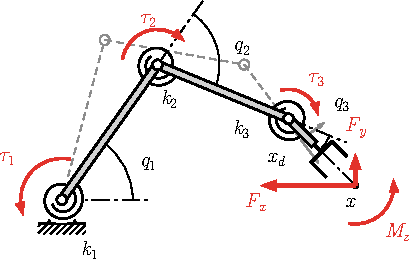
\includegraphics[width=\textwidth]{figures/JointImpendanceControllerModel.pdf}
        \caption{Joint-space impedance.}
        \label{fig:impedance-model-joint}
    \end{subfigure}\hfill
    \begin{subfigure}[b]{0.49\textwidth}
        \centering
        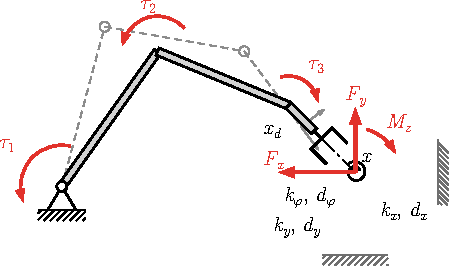
\includegraphics[width=\textwidth]{figures/ImpendanceControllerModel.pdf}
        \caption{Operational-space impedance.}
        \label{fig:impedance-model-task}
    \end{subfigure}
    \caption{Impedance control, illustrated on a planar arm with three joints. (a) A virtual spring and damper with stiffness $k_1,k_2,k_3$, the diagonal entries of $\mat{K}_q$, act directly on each joint, pulling it toward its reference $q_{\mathrm{ref}}$. (b) A virtual spring and damper with stiffness $k_x,k_y,k_\varphi$ and damping $d_x,d_y,d_\varphi$, the diagonal entries of $\mat{K}_p$ and $\mat{K}_d$, act on the controlled end-effector frame along each task direction instead. The resulting wrench $(F_x,F_y,M_z)$ is mapped to the joint torques $\tau_1,\tau_2,\tau_3$ through $\mat{J}^{\mathrm{T}}$.}%
    \label{fig:impedance-model}%
\end{figure}%

The nullspace projector decides how strongly the posture term interferes with the task. It is dynamically consistent when $\mat{N}^{\mathrm{T}}=\mat{I}-\mat{J}^{\mathrm{T}}\bar{\mat{J}}^{\mathrm{T}}$ with the inertia-weighted pseudoinverse $\bar{\mat{J}}=\mat{M}^{-1}\mat{J}^{\mathrm{T}}(\mat{J}\mat{M}^{-1}\mat{J}^{\mathrm{T}})^{-1}$ and joint-space inertia $\mat{M}$~\cite{Dietrich2015,RoboticSystemsLab2019}. Torques in the nullspace then produce no acceleration of the controlled frame. A projector built from a pseudoinverse of the Jacobian without inertia weighting needs no inertia model, but it decouples the nullspace from the task only statically, so that posture torques can still disturb the task during motion~\cite{Dietrich2015}. The controllers in simulation and on the physical robot both use the dynamically consistent projector (Section~\ref{sec:setup}). Equation~\eqref{eq:osc} is the Factory and FORGE controller~\cite{Narang2022,Noseworthy2025}. Scaling the spring and damper term by the task-space inertia $\mat{\Lambda}=(\mat{J}\mat{M}^{-1}\mat{J}^{\mathrm{T}})^{-1}$ and compensating the nonlinear dynamics yields the full operational-space formulation, in which the closed loop becomes a decoupled unit-mass system in every task direction~\cite{Lynch2017}.

\section{Simulation Settings and Domain Randomization}\label{sec:app-sim}

\subsection{Simulator and Physics Settings}

Table~\ref{tab:sim-params} lists the simulator, thread-model, and hand settings of the teacher environment.

\begin{table}[!htbp]%
    \centering%
    \caption{Simulation settings, thread model, and simulated hand of Section~\ref{sec:teacher}.}%
    \label{tab:sim-params}%
    \small
\begin{tabularx}{\textwidth}{lY}
        \toprule
        Parameter & Value \\
        \midrule
        simulator & Isaac~Sim~5.1, Isaac~Lab~2.3.2, PhysX \\
        physics rate / policy rate & 120\,Hz / 15\,Hz (one command held over eight physics steps) \\
        \midrule
        prismatic thread drive & stiffness $2\times10^{5}$\,N/m, damping 200\,N\,s/m, force limit 1000\,N \\
        thread friction \eqref{eq:friction} & $\tau_c=2\times10^{-3}$\,N\,m, $c_v=2\times10^{-4}$\,N\,m\,s/rad, $\omega_s=0.1$\,rad/s \\
        thread pitch $\rho$ & 3.0 / 3.5 / 4.0\,mm for M24 / M30 / M36 \\
        nut carrier mass & 1\,g \\
        prismatic lower limit & 0.2\,mm above the physical stop \\
        \midrule
        pinch-joint effort limit & 0.5\,N\,m (other proximal hand joints 1.864\,N\,m, distal follower joints 50\,N\,m) \\
        pad friction coefficient & 1.5 nominal, randomized (Table~\ref{tab:dr}); robot 0.75, nut 1.0 \\
        \midrule
        arm joint dynamics & identified \ac{FR3}: friction 0.2\,N\,m, armature 0.195\,kg\,m$^{2}$, damping 0.003\,N\,m\,s/rad per joint \\
        joint-limit guard & episode ends when an arm joint is within 0.15\,rad of its limit \\
        reset pose & hand wound $45\degree$ about the bolt against the threading direction and tilted $30\degree$ wrist-up; bolt on the hardware holder \\
        \bottomrule
    \end{tabularx}
\end{table}%

The pinch-joint effort limit bounds the grip force. A replay of a policy trained without the limit gave median pad forces of about 43\,N at the thumb and 38\,N at the index. Limits of 1.0\,N\,m and 0.3\,N\,m reduced them to about 27/21\,N and 12/7\,N, whereas 0.1\,N\,m let the grip collapse. The retained limit of 0.5\,N\,m lies between the two working values.

\subsection{Teacher Observations}\label{sec:app-teacher-obs}

Table~\ref{tab:teacher-obs} lists the actor and critic observations of the teacher of Section~\ref{sec:teacher-training}. Each fingertip force channel is the force that the thumb or index pad exerts along its pad normal, computed from the total contact force on the pad, because the physical fingertip sensors observe neither the other force components nor which body presses on them. Each torque channel is the reaction torque at one arm joint, normalized by the effort limit of that joint.

\begin{table}[!htbp]%
    \centering%
    \caption{Actor and critic observations of the single-size M24 threading teacher. Noise is applied to the actor only. Joint torques are divided by the effort limits of 87\,N\,m (joints 1--4) and 12\,N\,m (joints 5--7).}%
    \label{tab:teacher-obs}%
    \small
\begin{tabularx}{\textwidth}{lYcY}
        \toprule
        Input & Component & Dim & Noise (actor) \\
        \midrule
        actor (46-D) & fingertip position relative to bolt frame & 3 & $\mathcal{N}(0,0.5\,\mathrm{mm})$ per axis; bolt frame $\mathcal{N}(0,2\,\mathrm{mm})$ per reset \\
         & fingertip quaternion (WXYZ, $w$ and $z$ zeroed) & 4 & random-axis angle $\mathcal{N}(0,0.2\degree)$ \\
         & end-effector linear velocity & 3 & finite difference of noisy position \\
         & end-effector angular velocity ($x$ and $y$ zeroed) & 3 & finite difference of noisy quaternion \\
         & fingertip position relative to held nut & 3 & $\mathcal{N}(0,0.5\,\mathrm{mm})$ per axis, each body \\
         & held-nut quaternion (WXYZ) & 4 & random-axis angle $\mathcal{N}(0,0.2\degree)$ \\
         & target position error & 3 & inherits nut noise \\
         & target quaternion error (WXYZ, $w\geq0$) & 4 & inherits nut noise \\
         & grasp-phase flag & 1 & none \\
         & thumb / index flexion force & 2 & gain $U(0.6,1.4)$, offset $U(-2,2)$\,N per reset; $\mathcal{N}(0,2\,\mathrm{N})$; $\ge0$ \\
         & arm joint torques (normalized) & 7 & gain $U(0.8,1.2)$, offset $U(-0.02,0.02)$ per reset; $\mathcal{N}(0,0.01)$; in $[-1,1]$ \\
         & previous filtered action (roll, pitch masked) & 9 & none \\
        \midrule
        critic (76-D) & fingertip position, quaternion, velocities & 13 & clean \\
         & arm joint positions & 7 & clean \\
         & held-nut position, position relative to bolt, quaternion & 10 & clean \\
         & bolt position and quaternion & 7 & clean \\
         & controller proportional gains & 6 & sampled per reset \\
         & action smoothing factor & 1 & sampled per reset \\
         & thumb / index flexion force & 2 & clean \\
         & arm joint torques (normalized) & 7 & clean \\
         & position and rotation action thresholds & 6 & sampled per reset \\
         & target position, quaternion, progress & 8 & clean \\
         & previous filtered action (roll, pitch masked) & 9 & none \\
        \bottomrule
    \end{tabularx}
\end{table}%

\subsection{Domain Randomization}\label{sec:app-dr}

Table~\ref{tab:dr} lists the domain randomization. A per-episode offset of the bolt frame models calibration error and forces the teacher to close the loop on the nut rather than on the bolt frame. The friction, thread, arm-dynamics, and start-pose randomization starts at nominal values and reaches its full range when the initial-yaw curriculum reaches $\pm30\degree$. Once the curriculum is complete, the required success hold grows from eight to twelve steps (0.53\,s to 0.8\,s).

\begin{table}[!htbp]%
    \centering%
    \caption{Domain randomization during teacher training. $U(a,b)$ denotes uniform sampling. Multiplicative factors are sampled as $1+U(0,\ell)$ or its reciprocal with equal probability. Joint torques are in units of the joint effort limits. Quantities marked $\dagger$ start at their nominal value and widen to the listed range with the initial-yaw curriculum.}%
    \label{tab:dr}%
    \small
    \begin{tabularx}{\textwidth}{lYY}
        \toprule
        Group & Quantity & Range \\
        \midrule
        physics & nut mass offset & $U(-5,5)$\,g per reset \\
         & bolt static friction & $U(0.25,1.25)$, 128 buckets, once per environment \\
         & nut friction / finger pad friction$^{\dagger}$ & $U(0.6,1.4)$ / $U(1.0,2.0)$, once per environment \\
         & thread resistance$^{\dagger}$ & $\times$ log-uniform in $[0.25,4]$ on the Coulomb and viscous terms \\
         & arm joint friction / armature / damping$^{\dagger}$ & $\times U(0.8,2.0)$ / $\times U(0.7,1.3)$ / $\times U(0.7,1.3)$ of the nominal values \\
        controller & proportional gains & multiplicative, $\ell=0.41$, per axis and reset \\
         & action smoothing factor & $U(0.025,0.1)$ per reset; fingers $3\times$, capped at 1 \\
         & position / rotation threshold & multiplicative, $\ell=0.25$ / $0.29$ \\
         & dead zone & $U(0,[5,5,5,1,1,1])$ N, N\,m, resampled every 2\,s \\
        observation & fingertip and nut position & $\mathcal{N}(0,0.5\,\mathrm{mm})$ per axis and step \\
         & fingertip and nut orientation & random-axis angle $\mathcal{N}(0,0.2\degree)$ \\
         & fingertip quaternion & random sign flip \\
         & bolt frame & $\mathcal{N}(0,2\,\mathrm{mm})$ per axis and reset \\
         & fingertip forces & gain $U(0.6,1.4)$, offset $U(-2,2)$\,N per reset; $\mathcal{N}(0,2\,\mathrm{N})$ per step; $\ge0$ \\
         & arm joint torques & gain $U(0.8,1.2)$, offset $U(-0.02,0.02)$ per reset; $\mathcal{N}(0,0.01)$ per step; in $[-1,1]$ \\
        reward & pad-force penalty threshold & $U(5,10)$\,N per reset \\
        initial state & table pose & $U(-5,5)$\,cm in $x$, $U(-10,10)$\,cm in $y$, $U(-2.5,2.5)\degree$ yaw \\
         & nut yaw & curriculum $0\rightarrow\pm30\degree$ in $5\degree$ steps at 80\,\% success \\
         & nut axial height & $U(0,20)$\,mm below nominal, room for $65\degree$ reserved \\
         & bolt position$^{\dagger}$ & $U(-5,5)$\,cm in $x$ and $y$ \\
         & arm start pose$^{\dagger}$ & $U(-3,3)$\,cm per axis, $U(-10,10)\degree$ yaw of the grasp frame \\
        task & target turn $\theta^{*}$ & $U(55\degree,65\degree)$ per episode \\
        \bottomrule
    \end{tabularx}
\end{table}%

\subsection{Task-Wrench Dead Zone}\label{sec:app-ctrl-dz-train}

\paragraph{Purpose and implementation.} The teacher is trained with a dead zone on the task wrench, which models the unreliability of the controller at low forces. Let $\vec{w}=\mat{K}_p\vec{e}-\mat{K}_d\dot{\vec{x}}$ be the task wrench of \eqref{eq:osc} in the robot base frame and $\vec{d}\in\R^6_{\ge0}$ the thresholds. Each component is shrunk toward zero,
\begin{equation}\label{eq:dead-zone}
  \tilde{w}_i=\begin{cases}0, & |w_i|<d_i,\\ \operatorname{sign}(w_i)\,(|w_i|-d_i), & \text{otherwise,}\end{cases}\qquad i=1,\dots,6,
\end{equation}
and $\tilde{\vec{w}}$ replaces $\vec{w}$ in $\mat{J}^{\mathrm{T}}\vec{w}$. The nullspace term is not affected. The thresholds are drawn as $\vec{d}\sim U(\vec{0},\vec{d}_{\max})$ with $\vec{d}_{\max}=[5,5,5\,\mathrm{N},1,1,1\,\mathrm{N\,m}]$ at every reset and again every 2\,s, when they are redrawn for all environments at once. The training arm has gravity disabled. Recipes with physics randomization also add joint friction, scaling a nominal 0.2\,N\,m per joint by a factor from $U(0.8,2.0)$.

At the nominal gains of Table~\ref{tab:controller}, the worst-case thresholds correspond to a band of $5/565=8.8$\,mm in position and $1/28\,\mathrm{rad}=2.0\degree$ in orientation, inside which the spring produces no wrench. With zero position error, a pure damping wrench is also removed below $5/47.5=0.105$\,m/s and $1/10.6=0.094$\,rad/s.

\paragraph{Recipes.} Three dataset recipes treat the dead zone differently:
\begin{itemize}
  \item the \emph{extended-randomization} recipe inherits the teacher's dead zone together with gain noise ($\ell=0.41$), a random smoothing factor $U(0.025,0.1)$, the arm joint friction factor $U(0.8,2.0)$, and nut-depth randomization.
  \item the \emph{proprio-friction} recipe sets the dead zone to zero, fixes the gains and the smoothing factor at 0.0625, and keeps the joint friction factor $U(0.8,2.0)$.
  \item the \emph{return-dead-zone} student adds a dead zone only during release and return. It is drawn per return and per axis from zero to a configured maximum and set back to zero when the arm is handed back to the policy.
\end{itemize}

\section{Teacher Reward and Scripted Transitions}\label{sec:app-reward}

\subsection{Reward}

Table~\ref{tab:reward} lists the reward terms of the threading teacher, and the text below it defines the grasp condition and the terminations.

\begin{table}[!htbp]%
    \centering%
    \caption{Reward terms of the threading teacher \eqref{eq:reward}. Progress terms pay only for newly achieved progress. The weight of $P^{\mathrm{wrench}}$ rises from zero at the first initial-yaw curriculum level to one at its full range.}%
    \label{tab:reward}%
    \small
\begin{tabularx}{\textwidth}{lYl}
        \toprule
        Term & Definition & Weight \\
        \midrule
        $R^{\mathrm{center}}$ & newly achieved fraction of the initial grasp-center--nut-center gap, until the grasp latches & 30 \\
        $R^{\mathrm{face}}$ & newly achieved fraction of the initial pad--face gap, until the grasp latches & 30 \\
        $R^{\mathrm{grasp}}$ & one-time bonus when the proper grasp has held for 10 consecutive steps & 180 \\
        $R^{\mathrm{hold}}$ & per step with proper grasp and both pads pressing with at least 1\,N & 0.24 \\
        $R^{\mathrm{turn}}$ & newly achieved fraction of the keypoint distance to the target pose remaining at latch, while the grasp is live & 72 \\
        $R^{\mathrm{target}}$ & one-time bonus on success & 300 \\
        \midrule
        $P^{\mathrm{magnitude}}$ & normalized commanded translation and yaw & $10^{-3}$ \\
        $P^{\Delta a}$ & action change & 0.1 \\
        $P^{\mathrm{align}}$ & misalignment of hand and nut frames & 0.02 \\
        $P^{\mathrm{force}}$ & magnitude of the vector sum of the two pad contact forces above a threshold $U(5,10)$\,N, per newton & 0.05 \\
        $P^{\mathrm{settle}}$ & $\omega_t^2$ from $50\degree$ of rotation onward & 0.25 \\
        $P^{\mathrm{wrench}}$ & lateral force above 2\,N and axial force above 5\,N per newton, tilting torque above 0.05\,N\,m per N\,m & 0.05 / 0.05 / 1.0 \\
        $P^{\mathrm{clear}}$ & squared normalized violation of a 3\,cm arm--table clearance & 2.0 \\
        $P^{\mathrm{contact}}$ & arm--table contact force above 2\,N, per newton & 0.05 \\
        $P^{\mathrm{limit}}$ & barrier on each arm joint from 0.5\,rad of headroom down to the 0.15\,rad guard & 0.5 (per joint and step at the guard) \\
        \bottomrule
    \end{tabularx}
\end{table}%

A proper grasp is simultaneous thumb and index contact within 1\,cm of the designated faces, with opposing pad forces and a pinch line perpendicular to the nut axis. Besides success and the time limit, an episode terminates when the nut leaves the bolt by more than 3\,cm, tilts by more than $60\degree$, or releases the thread, when an arm joint comes within 0.15\,rad of its limit or trips the joint-velocity reflex, when no finger is in contact for more than 150 steps, when the thread model fails numerically, or when the latched grasp is lost. Each promotion of the success-hold curriculum requires a success rate of at least 80\,\% over completed episodes and at least five episode lengths since the previous change.

\subsection{Scripted Transitions}\label{sec:app-hybrid}

Table~\ref{tab:hybrid-params} lists the thresholds and timings of the scripted release and return that chain the teacher into the hybrid teacher.

\begin{table}[!htbp]%
    \centering%
    \caption{Thresholds and timings of the scripted transitions of the hybrid teacher (Section~\ref{sec:hybrid}).}%
    \label{tab:hybrid-params}%
    \small
    \begin{tabular}{lp{0.68\textwidth}}
        \toprule
        Parameter & Value \\
        \midrule
        release trigger & nut rotation within $5\degree$ of the target turn \\
        release waypoints & 4, interpolated over 0.73, 0.53, 0.60, and 1.00\,s (11, 8, 9, and 15 control steps) \\
        return segment & 1.07\,s (16 control steps) \\
        return gate & grasp frame within a tolerance drawn per return between 5 and 15\,mm and between $5\degree$ and $10\degree$, hand joints within 0.15\,rad; once 2.5\,s have passed, also accepted inside the upper limits \\
        transition pose clip & 0.05\,m and 0.25\,rad per axis on release and return rows (policy rows: 0.02\,m, 0.097\,rad) \\
        transition dead zone & task space, drawn per transition up to 7.5\,N and 1\,N\,m \\
        return timeout & 16\,s (transition failure) \\
        target turn clamp & $[55\degree,65\degree]$ \\
        \bottomrule
    \end{tabular}
\end{table}%

\section{Demonstration Dataset}\label{sec:app-data}

Table~\ref{tab:datasets} summarizes the ten-cycle M24 demonstrations from which the reported students are trained.

\begin{table}[!htbp]%
    \centering%
    \caption{Demonstration data of the M24 ten-cycle collection used for the reported students.}%
    \label{tab:datasets}%
    \small
\begin{tabularx}{\textwidth}{lY}
        \toprule
        Property & Value \\
        \midrule
        teacher & single-size M24 teacher of Section~\ref{sec:teacher}, mean action, $\beta=1$ \\
        simulated demonstrations & 36 successful ten-cycle episodes from one rollout of 16 parallel environments (6400 control steps, seed 1; 14 environments contributed) \\
        frames (15\,Hz) & 53\,408 (per episode 1341 / 1474 / 1838 min / median / max) \\
        cycle rollback & failed cycle retried from the last completed return, at most 3 times; 20 episodes contain a retried cycle, 10\,136 rows dropped in total \\
        start state & nominal pose, no initial yaw, nut at the top of the thread \\
        per-cycle target & $60\degree$ grid, release $5\degree$ before the target \\
        task randomization & none: nut mass, nut, bolt, and thread friction, arm joint armature and damping, controller parameters, nut-pose and bolt-frame observation noise, start poses, and target turn fixed at nominal values \\
        proprioception noise & fingertip pose $\mathcal{N}(0,0.5\,\mathrm{mm})$ and $\mathcal{N}(0,0.2\degree)$ per step; fingertip forces gain $U(0.6,1.4)$, offset $U(-2,2)$\,N per episode, $\mathcal{N}(0,2\,\mathrm{N})$ per step; arm joint torques gain $U(0.8,1.2)$, offset $U(-0.02,0.02)$ per episode, $\mathcal{N}(0,0.01)$ per step, in units of the effort limits \\
        joint and pad friction & arm joint friction scaled by $U(0.8,2.0)$, finger pad friction $U(1.2,1.8)$, once per environment \\
        camera pose & per episode, uniform per axis within $\pm11.2$\,mm and $\pm1.13\degree$ \\
        release and return & thresholds, clip, and dead zone of Table~\ref{tab:hybrid-params} \\
        impulses per episode & 30 (one per policy, waypoint, and return segment), 0.05--0.25\,N\,s, 0.05--0.20\,s after segment start \\
        visual randomization & dome light, table, nut/bolt, floor textures, background \\
        material sampling & per environment and reset, roughness $U(0.3,0.9)$, metallicity $U(0,0.15)$ \\
        dome light and floor & shared, redrawn with $p=0.3$ per reset, light intensity $U(1000,4000)$ \\
        background image & $p=0.5$ per environment and reset, replaces pixels at 1.5\,m or beyond or without depth \\
        image size & $320\times180$ RGB and metric depth ($640\times480$ sensor, centered $640\times360$ crop, downscaled by two) \\
        \bottomrule
    \end{tabularx}
\end{table}%
